\chapter{Evaluation}\label{evaluation}
This chapter starts by evaluating the proposed neural network architectures on CPUs and GPUs to find a baseline inference latency, accuracy and AUC values. This information is then compared with the results obtained from simulating and synthesizing the models on reconfigurable hardware. The outcome of the design space exploration includes hardware resource utilization metrics as well as discussion about the Pareto front, applicability in high energy physics environments, and verification of the analytical models formulated in the previous chapter. Lastly, both the quantization-aware training and post-training quantization are evaluated quantitatively in terms of the trade-off between quality of results and bit-width reduction as well as qualitatively for their ease of adaptation to existing designs.

As efficient hardware mapping is the motivation behind the proposed models, out of the constituent list representation datasets, only the one containing 30 most energetic jets is analyzed in this chapter due to the inherent complexity of transformer neural networks and the challenges involved in mapping bigger designs to FPGAs.

\section{Proposed Models' Performance}
The first objective of the project is to design neural network architectures capable of very fast and accurate classification. Firstly, the classification accuracies and ROC curves are analyzed. Then, the choice of a dataset for both models is discussed, followed by inference latency results and comparison to existing solutions.

\subsection{Classification Accuracy}
Table \ref{tab:classification-results} shows the evaluation results of the base and the two proposed architectures on the HLF and the constituent list datasets. Compared to the base one, the ultra-low latency model requires roughly 156 times fewer parameters and 2,875 times fewer FLOPS while achieving comparable classification results, suggesting that the base model has significantly too much learning capacity for that dataset. The second model also offers a notable parameters and FLOPS reduction of around 4 times. This matches the quadratic complexity of the self-attention layer given that the latent dimension is reduced from \(128\) to \(64\) and proves the importance of this factor. Along this, there is a slight improvement in accuracy and AUC thanks to a more careful selection of the design parameters.

\begin{table}[hpt!]
  \centering
  \caption{Comparison between classification accuracy, average ROC metrics, parameter count, and FLOPS between the baseline and the proposed architectures.}
  \label{tab:classification-results}
  \bgroup
  \def\arraystretch{1.2}
  \setlength\tabcolsep{2.5mm}
  \begin{tabular}{|c|c|c|c|c|c|}
  \hline
  \textbf{Architecture} & \textbf{Dataset} & \textbf{\begin{tabular}[c]{@{}c@{}}Classification\\ Accuracy (\%)\end{tabular}} & \textbf{AUC} & \textbf{Parameters} & \textbf{FLOPS} \\ \hline \hline
  Base & \multirow{2}{*}{HLF} & 76.50 & 0.9429 & 399,901 & 102 M \\ \cline{1-1} \cline{3-6} 
  Ultra-Low Latency &  & 76.09 & 0.9396 & 2,605 & 583 k \\ \hline
  Base & \multirow{2}{*}{\begin{tabular}[c]{@{}c@{}}Constituents\\ (30)\end{tabular}} & 77.56 & 0.9473 & 405,643 & 1,676 M \\ \cline{1-1} \cline{3-6} 
  Accuracy-Focused &  & 77.81 & 0.9480 & 107,403 & 448 M \\ \hline
  \end{tabular}
  \egroup
  \end{table}

\subsection{Receiver Operating Characteristic Curves and their Areas}
Analyzing the ROC curves offers a more complex analysis of the trade-offs in classification results between the base and the proposes architecture.

\indo{confusion matrix}

\begin{figure}[!hpt]
  \centering
  \begin{tabular}{ccc}
      {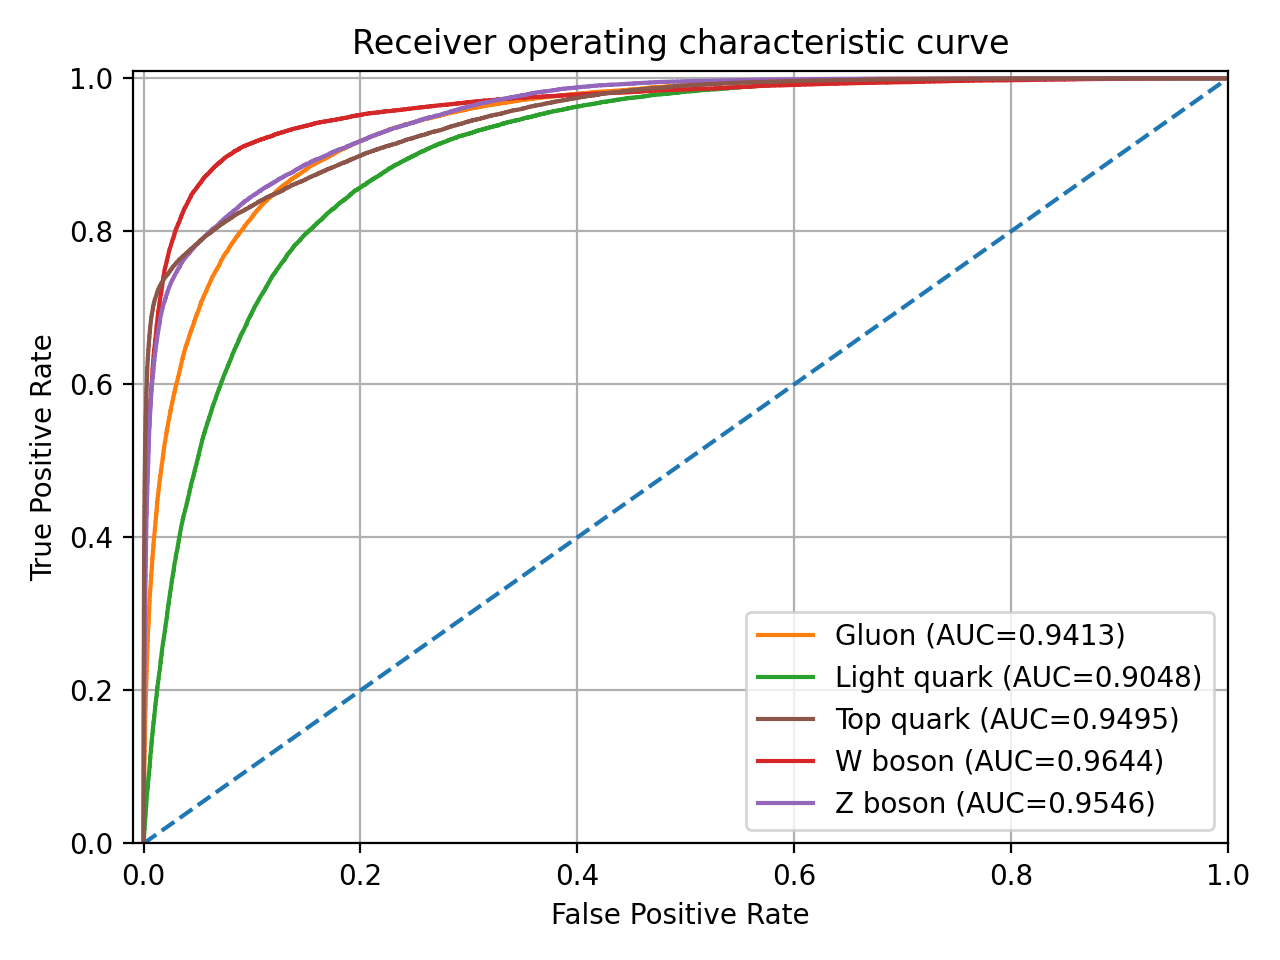
\includegraphics[width=0.48\columnwidth]{evaluation/ROC_base_hlf.png}} &
      {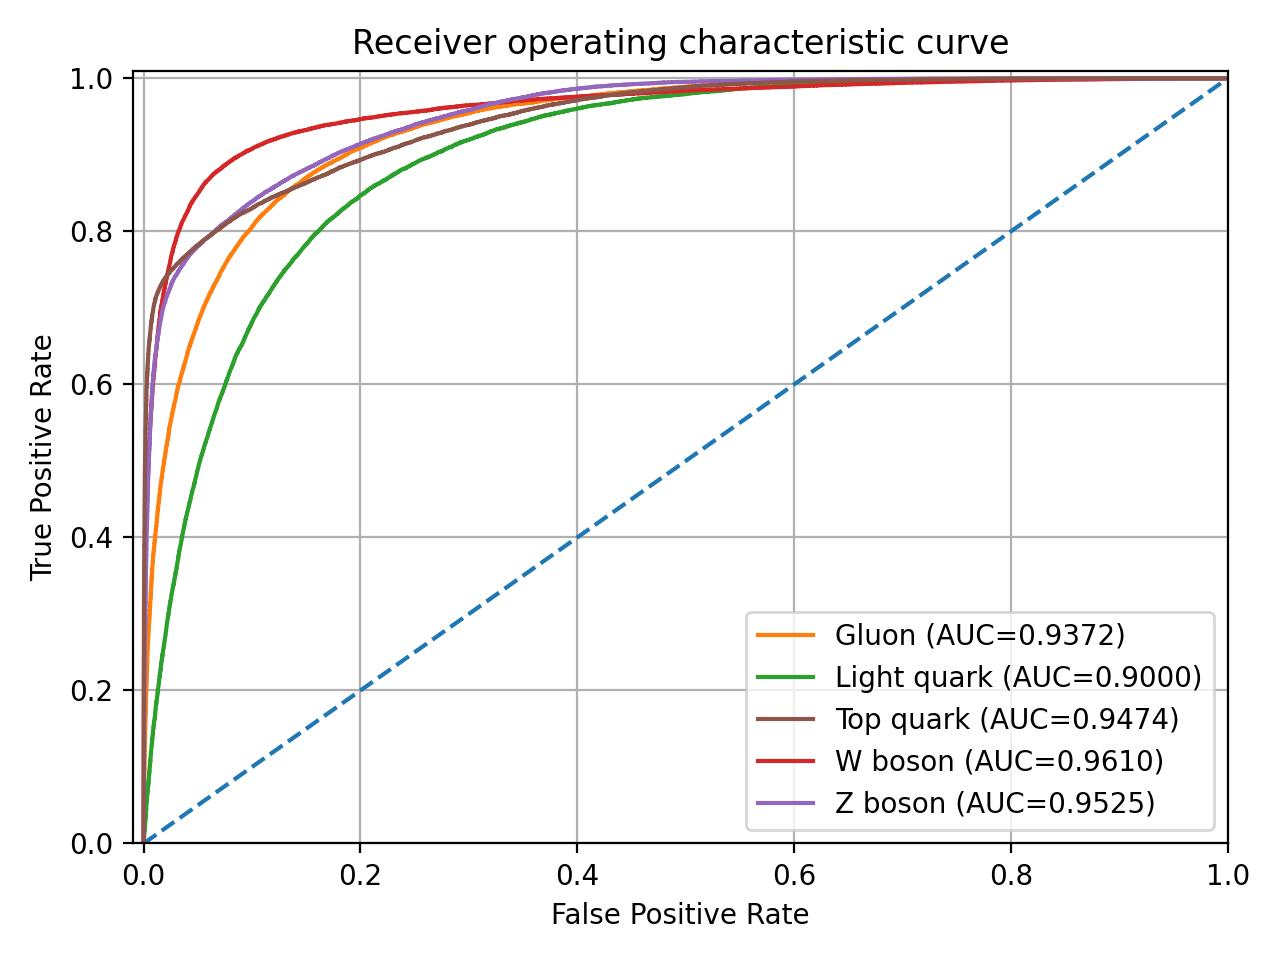
\includegraphics[width=0.48\columnwidth]{evaluation/ROC_hlf.png}}
  \end{tabular}
  \caption{Comparison between ROC and AUC of the base (left) and ultra-low latency (right) models using the HLF dataset.}
  \label{fig:ROCs-HLF}
\end{figure}

Figure \ref{fig:ROCs-HLF} compares the base and the ultra-low latency models trained on the HLF dataset. The curves behave very similarly, with the ones associated with gluons and light quarks achieving notably lower true positive rates (TRPs) at lower false positive rates (FPRs), which means that both models have more troubles between distinguishing between these two jet categories.

\begin{figure}[!hpt]
  \centering
  \begin{tabular}{ccc}
      {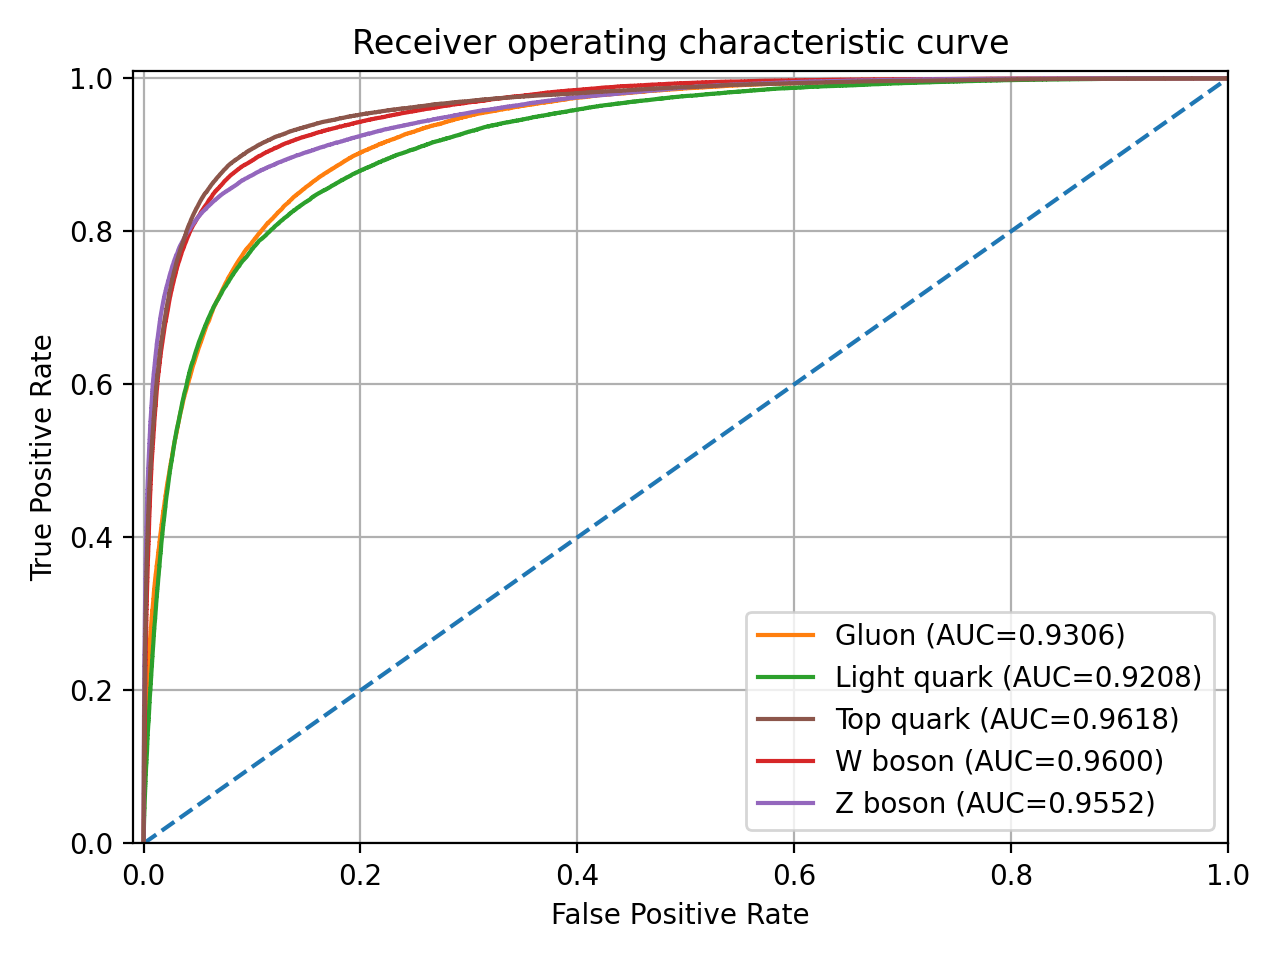
\includegraphics[width=0.48\columnwidth]{evaluation/ROC_base_constituent.png}} &
      {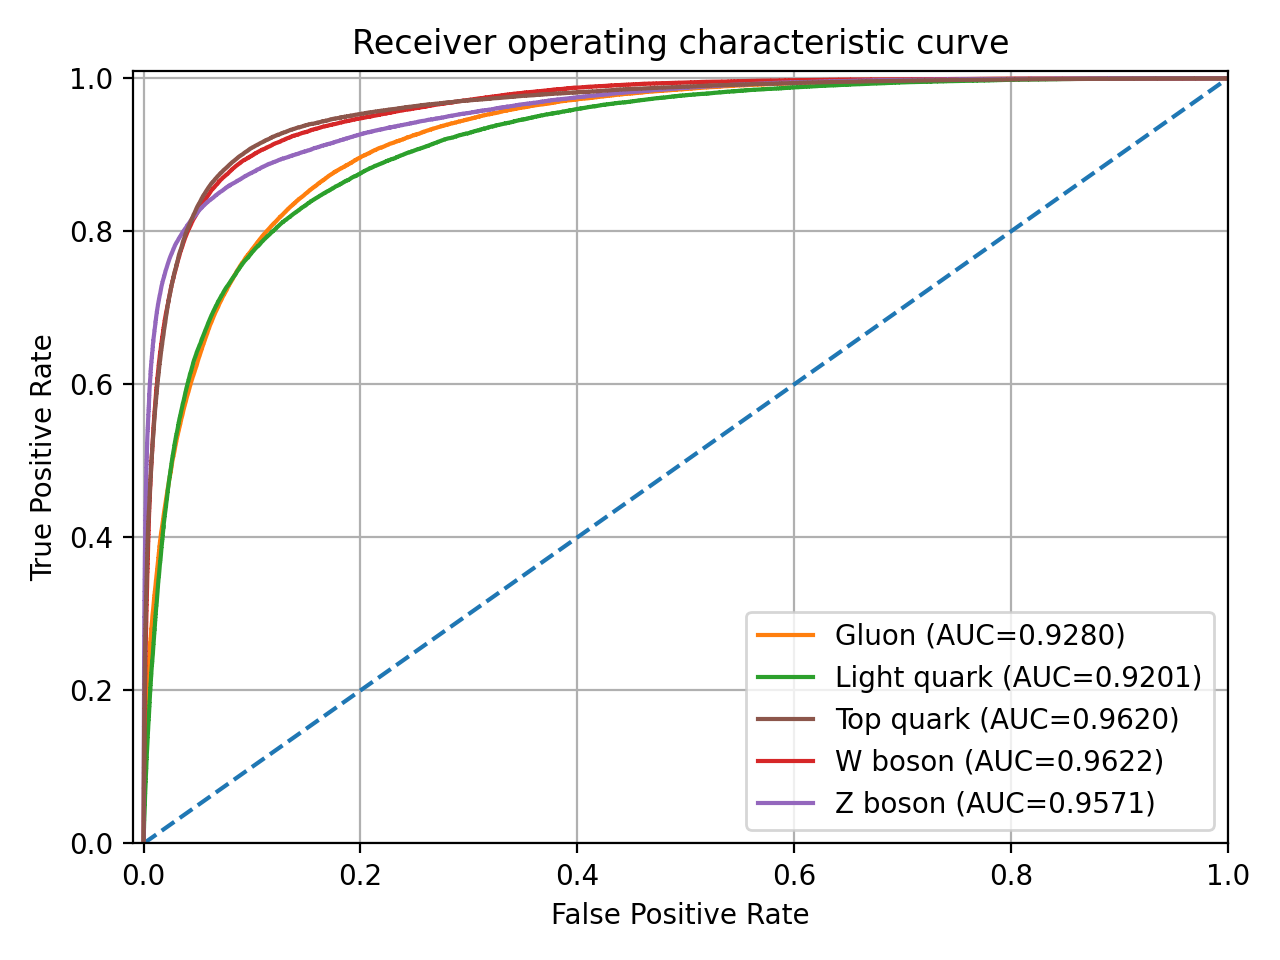
\includegraphics[width=0.48\columnwidth]{evaluation/ROC_constituent.png}}
  \end{tabular}
  \caption{Comparison between ROC and AUC of the base (left) and accuracy-focused (right) models using the constituent list dataset.}
  \label{fig:ROCs-constituent}
\end{figure}

Figure \ref{fig:ROCs-constituent} shows an analogous comparison for the base and accuracy-focused models using the constituent list representation. Gluons and light quarks' classifications are still behind the other jets, indicating the more challenging nature of differentiating between these jet categories.

\begin{table}[!hpt]
  \centering
  \caption{AUC and true positive rates at 10 \% and 1 \% false positive rates for the ultra-low latency and accuracy-focused models.}
  \label{tab:AUCs}
  \bgroup
  \def\arraystretch{1.2}
  \setlength\tabcolsep{2.5mm}
  \begin{tabular}{c|ccc|ccc|}
  \cline{2-7}
  \multicolumn{1}{l|}{} & \multicolumn{3}{c|}{\textbf{Ultra-low latency}} & \multicolumn{3}{c|}{\textbf{Accuracy-focused}} \\ \hline
  \multicolumn{1}{|c|}{\multirow{2}{*}{\textbf{Jet}}} & \multicolumn{1}{c|}{\multirow{2}{*}{\textbf{AUC}}} & \multicolumn{2}{c|}{\textbf{TPR @ FPR}} & \multicolumn{1}{c|}{\multirow{2}{*}{\textbf{AUC}}} & \multicolumn{2}{c|}{\textbf{TPR @ FPR}} \\ \cline{3-4} \cline{6-7} 
  \multicolumn{1}{|c|}{} & \multicolumn{1}{c|}{} & \multicolumn{1}{c|}{\textbf{10 \%}} & \textbf{1 \%} & \multicolumn{1}{c|}{} & \multicolumn{1}{c|}{\textbf{10 \%}} & \textbf{1 \%} \\ \hline \hline
  \multicolumn{1}{|c|}{Gluon} & \multicolumn{1}{c|}{0.9372} & \multicolumn{1}{c|}{0.8057} & 0.3928 & \multicolumn{1}{c|}{0.9280} & \multicolumn{1}{c|}{0.7765} & 0.3242 \\ \hline
  \multicolumn{1}{|c|}{Light quarks} & \multicolumn{1}{c|}{0.9000} & \multicolumn{1}{c|}{0.6813} & 0.1618 & \multicolumn{1}{c|}{0.9201} & \multicolumn{1}{c|}{0.7729} & 0.2788 \\ \hline
  \multicolumn{1}{|c|}{Top quark} & \multicolumn{1}{c|}{0.9474} & \multicolumn{1}{c|}{0.8304} & 0.7064 & \multicolumn{1}{c|}{0.9620} & \multicolumn{1}{c|}{0.9094} & 0.5553 \\ \hline
  \multicolumn{1}{|c|}{W boson} & \multicolumn{1}{c|}{0.9610} & \multicolumn{1}{c|}{0.9079} & 0.6207 & \multicolumn{1}{c|}{0.9622} & \multicolumn{1}{c|}{0.8990} & 0.5632 \\ \hline
  \multicolumn{1}{|c|}{Z boson} & \multicolumn{1}{c|}{0.9525} & \multicolumn{1}{c|}{0.8390} & 0.6277 & \multicolumn{1}{c|}{0.9571} & \multicolumn{1}{c|}{0.8768} & 0.6704 \\ \hline
  \end{tabular}
  \egroup
\end{table}

Table \ref{tab:AUCs} provides a comprehensive view of the models' true positive rates at 10 \% and 1 \% false positive rates. Interestingly, the ultra-low latency model yields a superior classification of gluons, despite being a simpler design. This can be attributed to the HLF dataset that might capture some characteristics of gluons better than the constituent list one.

\subsection{CPU and GPU Latency}
Table \ref{tab:inference-times-ultra-low-latency} and \ref{tab:inference-times-accuracy-focused} display the inference times for the two proposed models, measured on several CPUs and GPUs. The results serve as a baseline for quantifying the improvements thanks to the hardware acceleration, which are discussed in the next section. The experimental setup for accurately measuring the inference times involves firstly performing 5 warm-up runs, followed by CUDA-synchronization where applicable, and then timing 200 test runs, for which mean and standard deviation were calculated. It is worth pointing out that the results for the ultra-low latency model are similar regardless of the underlying hardware, including very little differences in performance between CPUs and GPUs. This can suggest that the machines are bottle-necked in terms of memory instead of computational resources, as that behavior is not observed for the more computationally-complex, accuracy-focused model.

\begin{table}[hpt!]
  \centering
  \caption{Comparison of ultra-low latency model's inference times, with batch size of 128}
  \label{tab:inference-times-ultra-low-latency}
  \bgroup
  \def\arraystretch{1.2}
  \setlength\tabcolsep{3mm}
  \begin{tabular}{c|l|cc|}
  \cline{2-4}
  \multicolumn{1}{l|}{}                               & \multicolumn{1}{c|}{\multirow{2}{*}{\textbf{Device}}} & \multicolumn{2}{c|}{\textbf{Inference time}}                      \\ \cline{3-4} 
  \multicolumn{1}{l|}{}                               & \multicolumn{1}{c|}{}                                 & \multicolumn{1}{c|}{per batch (ms)}          & per sample ($\mu$s) \\ \hline
  \multicolumn{1}{|c|}{\multirow{4}{*}{\textbf{\begin{sideways}CPU\end{sideways}}}} & Intel Xeon Silver 4110  & \multicolumn{1}{c|}{1.741 $\pm$ 0.027}       & 13.604 $\pm$ 0.207 \\ \cline{2-4} 
  \multicolumn{1}{|c|}{}                              & Intel Xeon X5690                                      & \multicolumn{1}{c|}{1.622 $\pm$ 0.026}       & 12.670 $\pm$ 0.206 \\ \cline{2-4} 
  \multicolumn{1}{|c|}{}                              & Intel Xeon E5-2620 v3                                 & \multicolumn{1}{c|}{1.325 $\pm$ 0.123}       & 10.350 $\pm$ 0.963 \\ \cline{2-4}
  \multicolumn{1}{|c|}{}                              & Intel Xeon Gold 6154                                  & \multicolumn{1}{c|}{1.167 $\pm$ 0.066}       & 9.112 $\pm$ 0.516  \\ \hline\hline
  \multicolumn{1}{|c|}{\multirow{3}{*}{\textbf{\begin{sideways}GPU\end{sideways}}}} & Nvidia GTX 1080 Ti      & \multicolumn{1}{c|}{1.166 $\pm$ 0.112}       & 9.111 $\pm$ 0.876  \\ \cline{2-4} 
  \multicolumn{1}{|c|}{}                              & Nvidia TITAN X                                        & \multicolumn{1}{c|}{1.154 $\pm$ 0.119}       & 9.017 $\pm$ 0.928  \\ \cline{2-4} 
  \multicolumn{1}{|c|}{}                              & Nvidia TITAN Xp                                       & \multicolumn{1}{c|}{1.062 $\pm$ 0.036}       & 8.296 $\pm$ 0.283  \\ \cline{2-4} 
  \hline
  \end{tabular}
  \egroup
\end{table}

The detailed specifications of the four machines used for measuring the inference time are listed below. All machines run CentOS 7.0 operating system, while the first listed machine, which is the GPU host, uses CUDA version 11.5, with driver version 495.29.05.

\begin{itemize}
  \item Dual Intel Xeon Silver 4110 at 2.10GHz with 192 GB DDR4 RAM at 2666 MT/s,
  \item Dual Intel Xeon X5690 at 3.47GHz with 96 GB DDR3 RAM at 1333 MT/s,
  \item Intel Xeon E5-2620 v3 at 2.40GHz with 192 GB DDR4 RAM at 2133 MT/s,
  \item Dual Intel Xeon Gold 6154 CPU at 3.00GHz with 768 GB DDR4 RAM at 2666 MT/s,
\end{itemize}

\begin{table}[hpt!]
  \centering
  \caption{Comparison of accuracy-focused model's inference times, with batch size of 128}
  \label{tab:inference-times-accuracy-focused}
  \bgroup
  \def\arraystretch{1.2}
  \setlength\tabcolsep{3mm}
  \begin{tabular}{c|l|cc|}
  \cline{2-4}
  \multicolumn{1}{l|}{}                               & \multicolumn{1}{c|}{\multirow{2}{*}{\textbf{Device}}} & \multicolumn{2}{c|}{\textbf{Inference time}}                      \\ \cline{3-4} 
  \multicolumn{1}{l|}{}                               & \multicolumn{1}{c|}{}                                 & \multicolumn{1}{c|}{per batch (ms)}          & per sample ($\mu$s) \\ \hline
  \multicolumn{1}{|c|}{\multirow{4}{*}{\textbf{\begin{sideways}CPU\end{sideways}}}} & Intel Xeon Silver 4110  & \multicolumn{1}{c|}{13.681 $\pm$ 0.087}       & 106.881 $\pm$ 0.678 \\ \cline{2-4} 
  \multicolumn{1}{|c|}{}                              & Intel Xeon X5690                                      & \multicolumn{1}{c|}{16.874 $\pm$ 0.237}       & 131.832 $\pm$ 1.851 \\ \cline{2-4} 
  \multicolumn{1}{|c|}{}                              & Intel Xeon E5-2620 v3                                 & \multicolumn{1}{c|}{15.311 $\pm$ 0.444}       & 119.616 $\pm$ 3.468 \\ \cline{2-4}
  \multicolumn{1}{|c|}{}                              & Intel Xeon Gold 6154                                  & \multicolumn{1}{c|}{7.436 $\pm$ 0.498}       & 58.092 $\pm$ 3.888  \\ \hline\hline
  \multicolumn{1}{|c|}{\multirow{3}{*}{\textbf{\begin{sideways}GPU\end{sideways}}}} & Nvidia GTX 1080 Ti      & \multicolumn{1}{c|}{2.941 $\pm$ 0.186}       & 22.975 $\pm$ 1.452  \\ \cline{2-4} 
  \multicolumn{1}{|c|}{}                              & Nvidia TITAN X                                        & \multicolumn{1}{c|}{3.258 $\pm$ 0.358}       & 25.456 $\pm$ 2.797  \\ \cline{2-4} 
  \multicolumn{1}{|c|}{}                              & Nvidia TITAN Xp                                       & \multicolumn{1}{c|}{2.993 $\pm$ 0.269}       & 23.385 $\pm$ 2.099  \\ \cline{2-4} 
  \hline
  \end{tabular}
  \egroup
\end{table}

\subsection{Comparison with Existing Solutions}
It is essential to compare the proposed architectures with recent state-of-the-art designs mentioned in \cref{background}. Table \ref{tab:all-networks-comparison} shows the key characteristics of each neural network architecture. Although the inference times were measured on different hardware platforms, it can be safely assumed that the overall trends are maintained given the results obtained in the previous subsection.

\begin{table}[!hpt]
  \centering
  \caption{Summary of networks' inference time, accuracy, Floating-Point Operations Per Second and parameter number for optimal batch sizes, with best values in bold. Inference times were measured using \textsuperscript{*}NVIDIA GTX 1080, \textsuperscript{$\dagger$}16-thread virtualized cloud CPU, \textsuperscript{$\ddagger$}NVIDIA GTX 1080 Ti.}
  \label{tab:all-networks-comparison}
  \bgroup
  \def\arraystretch{1.2}
  \setlength\tabcolsep{1.5mm}
  \begin{tabular}{|c|c|c|c|c|}
  \hline
  \textbf{\begin{tabular}[c]{@{}c@{}}Neural network\\ \end{tabular}} & \textbf{\begin{tabular}[c]{@{}c@{}}Inference per\\ batch (ms)\end{tabular}} & \textbf{\begin{tabular}[c]{@{}c@{}}Accuracy /\\ aver. AUC\end{tabular}} & \textbf{FLOPS} & \textbf{Parameters} \\ \hline \hline
  DNN \cite{9-newman2019jedi-net:} & \textbf{1.0 $\pm$ 0.2}\textsuperscript{*} & 0.760 / 0.941 & \textbf{27 k} & 14,725 \\ \hline
  CNN \cite{9-newman2019jedi-net:} & 57.1 $\pm$ 0.5\textsuperscript{*} & 0.740 / 0.911 & 400 k & 205,525 \\ \hline
  GRU \cite{9-newman2019jedi-net:} & 23.2 $\pm$ 0.6\textsuperscript{*} & 0.750 / 0.912 & 46 k & 15,575 \\ \hline
  JEDI-net \cite{9-newman2019jedi-net:} & 121.2 $\pm$ 0.4\textsuperscript{*} & TODO / 0.959 & 116 M & 33,625 \\ \hline
  JEDI-net with $\sum O$ \cite{9-newman2019jedi-net:}  & 402.0 $\pm$ 1.0\textsuperscript{*} & TODO / 0.957 & 458 M & 8,767 \\ \hline
  ConstituentNet-Base \cite{3-yuan2021constituentnet:} & $\sim$133.7\textsuperscript{$\dagger$} & 0.818 / \textbf{0.966} & 1,553 M & 289,000 \\ \hline
  ConstituentNet-Tiny \cite{3-yuan2021constituentnet:} & $\sim$12.4\textsuperscript{$\dagger$} & 0.805 / 0.960 & 13 M  & 8,533 \\ \hline \hline
  Ultra-Low Latency & 1.2 $\pm$ 0.1\textsuperscript{$\ddagger$} & 0.761 / 0.940 & 583 k & \textbf{2,605} \\ \hline
  Accuracy-Focused & 2.9 $\pm$ 0.2\textsuperscript{$\ddagger$} & 0.778 / 0.948 & 448 M & 107,403 \\ \hline
  \end{tabular}
  \egroup
\end{table}

It is important to mention that the accuracy and AUC values claimed in the literature are obtained thanks to an extensive hyperparameter tuning, which is beyond the scope of this project. Nonetheless, the proposed architectures offer an interesting trade-off between the quality of results and design complexity, which is highlighted by the low inference time.

\section{Hardware Acceleration}
This section covers the results of the hardware implementation of the two proposed architectures. It also discusses the design space exploration performed using C simulation and synthesis processes available in Vivado HLS. Thanks to its high-performance, Xilinx Virtex Ultrascale+ XCU250 (variant figd2104-2L-e) was chosen as the target FPGA platform. It contains 5,376 18 Kb BRAMs, 12,288 DSP slices, 3,456,000 registers (also referred to as FFs), and 1,728,000 LUTs.

\subsection{Ultra-Low Latency Model}
The first of the proposed models undergoes a series of optimization steps, with the aim of finding the fastest, yet still accurate design configuration. The steps are described below, with their impact on latency and resource utilization depicted in figure \ref{fig:hardware-optimizations}.

\begin{enumerate}
  \item Initial implementation of the architecture.
  \item SiLU activations are replaced by ReLU, leading to a slight latency improvement with a 6 \% decrease in BRAMs with no sigmoid functions needing precomputing.
  \item Pipelining is introduced, latency decreases nearly 1000 times, 5 times less BRAMs are needed thanks to array partitioning, but at the same time more DSPs, LUTs and FFs are instantiated to handle the parallelism.
  \item Dependencies in linear layers are simplified, which decreases all resources' utilization, but worsens latency.
  \item Separate instances of linear layers without bias calculation are used, which reduces LUTs and FFs usage, but surprisingly causes a slight increase in latency.
  \item More arrays are partitioned and some are explicitly set to LUTs instead of BRAMs, halving the number of the latter and reducing latency by over 40 \%.
  \item The optimized log softmax block replaces the naive implementation, which causes an 86 \% latency improvement with marginal resource utilization decrease.
  \item The \textit{queries}, \textit{keys}, and \textit{values} fully-connected block is split into separate layers, reducing BRAMs thanks to more optimal weights allocation and decreasing latency.
  \item Tensor product is reorganized and simplified, nearly halving latency and BRAMs, while notably reducing LUTs and FFs.
  \item Tensor product gets fully unrolled, which again halves the latency, but causes a noticeable increase in overall resource utilization.
  \item Top level module variables are reorganized to reduce FFs and LUTs usage.
  \item The uniform design bit-width is reduced to match DSP specification to allow for a more optimal routing, halving their required number and causing an overall improvement to latency and other resources.
\end{enumerate}

\begin{figure}[hpt!]
  \centering
  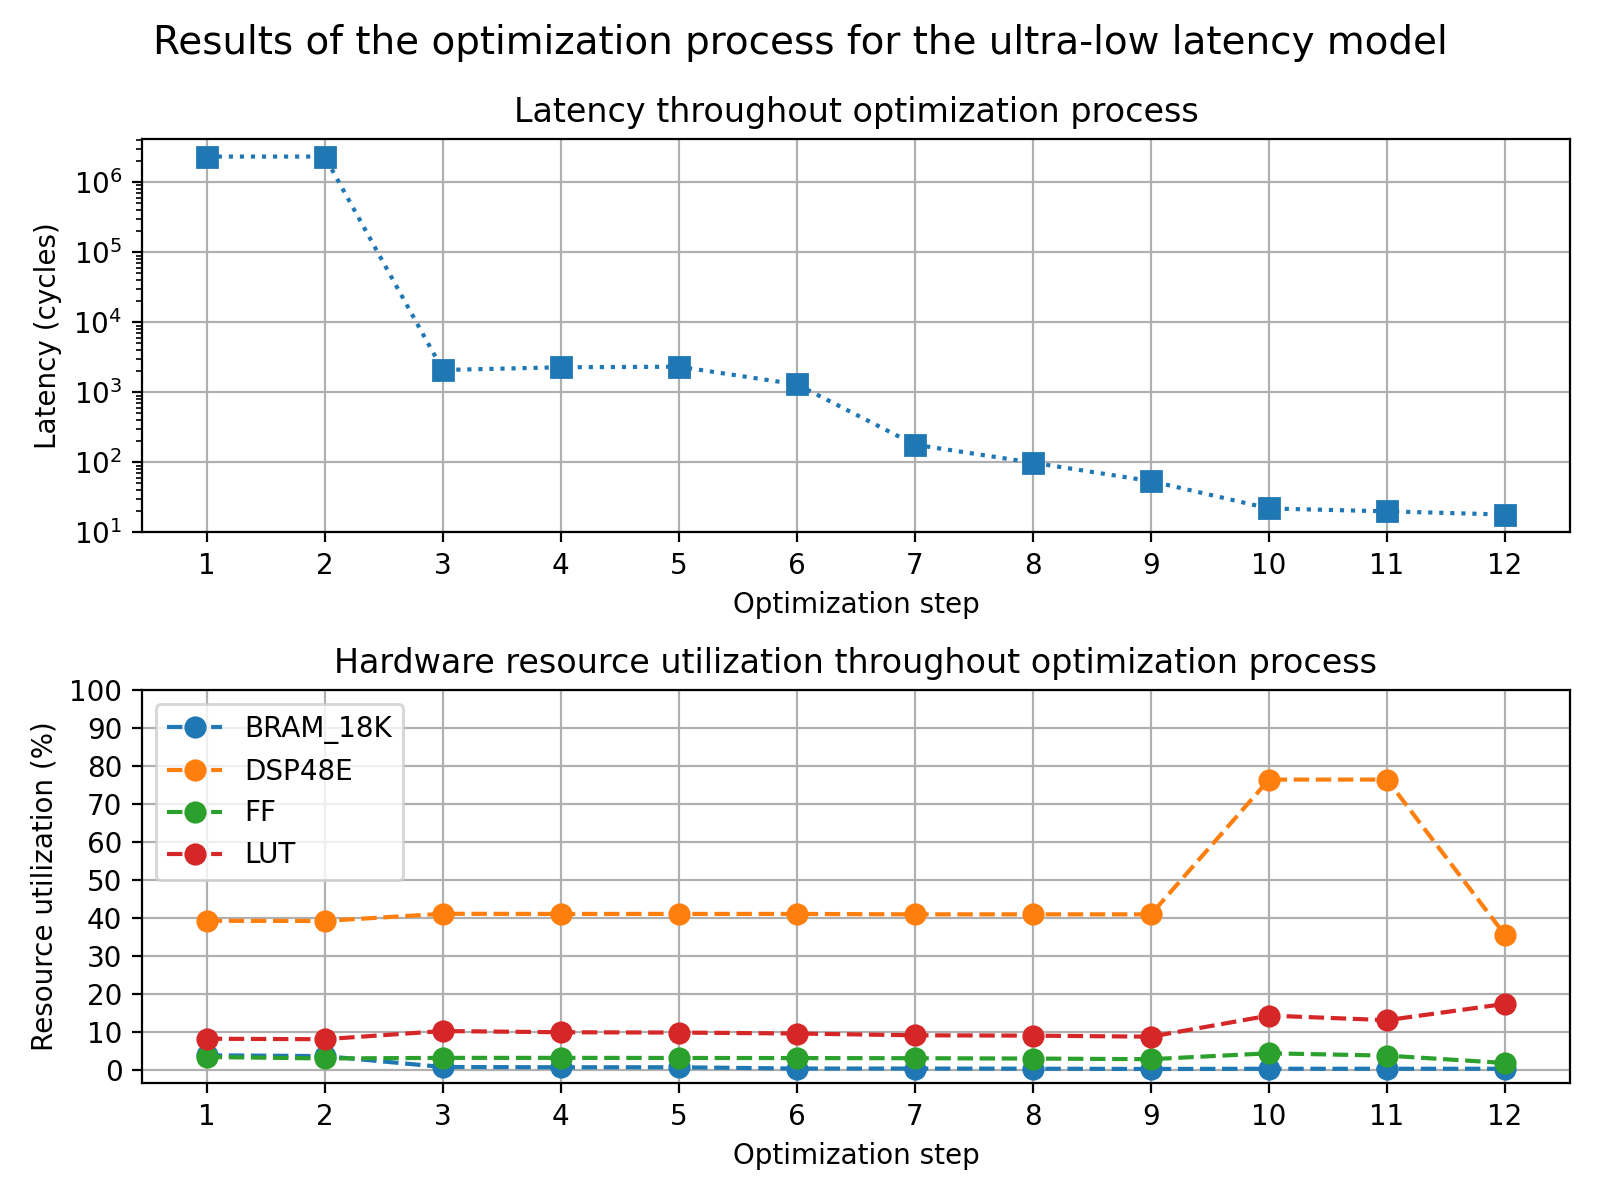
\includegraphics[trim={0cm 0cm 0cm 1cm}, clip, width=0.8\textwidth, center]{../logs/hardware_optimizations.png}
  \caption{Results of the optimization process for the ultra-low latency model.}
  \label{fig:hardware-optimizations}
\end{figure}

The final design's resource usage can be seen in figure \ref{tab:utilization}, while its timing results are shown in figure \ref{tab:fgpa-timing}. Overall, the optimization process leads to an over 1,000,000 times faster inference speed, with decreases in all resources aside from LUTs.

\begin{table}[hpt!]
  \centering
  \caption{FPGA resources utilization}
  \label{tab:utilization}
  \bgroup
  \def\arraystretch{1.3}
  \setlength\tabcolsep{3mm}
  \begin{tabular}{r|c|c|c|c|}
  \cline{2-5}
  \multicolumn{1}{c|}{}                      & \textbf{BRAM 18K} & \textbf{DSP48E} & \textbf{FF} & \textbf{LUT} \\ \hline
  \multicolumn{1}{|r|}{\textbf{Total used}}       & 12                 & 4,351            & 58,942       & 298,881       \\ \hline
  \multicolumn{1}{|r|}{\textbf{Available}}   & 5,376              & 12,288           & 3,456,000     & 1,728,000      \\ \hline\hline
  \multicolumn{1}{|r|}{\textbf{Utilization}} & 0.22\%            & 35.41\%         & 1.71\%      & 17.30\%       \\ \hline
  \end{tabular}
  \egroup
\end{table}

Along with the FPGA clock period of 5 ns\footnote{5 ns period corresponds to a frequency of 200 MHz, which is used at L1T at LHC.} with a 12.5 \% uncertainty, the final design is able to perform a successful inference in only 90 ns with adequate slack. Thus, the hardware acceleration leads to an over 500 times decrease in latency per sample compared to the CPU and GPU implementation, and it is well within the L1T 12.5 \(\mu s\) latency constraint, leaving a significant headroom for more complex processing. The test accuracy is measured as 74.4 \%, which is 1.7 percent point lower than the original floating-point implementation. The average AUC is slightly lower at 0.9368, with the quantization noise being considered as the main factor for the decrease is classification capability. These values are inline with other results obtained using \hlsml \cite{53-kreinar2018fast}, however, our implemented hardware model is over 4 times faster despite not undergoing any compression, pruning or quantization, which highlights the potential of the described optimization process.

\begin{table}[!hpt]
  \centering
  \caption{Information about design's clock, latency and initiation interval.}
  \label{tab:fgpa-timing}
  \bgroup
  \def\arraystretch{1.2}
  \setlength\tabcolsep{1.5mm}
  \begin{tabular}{|c|c|c||cc|c|}
  \hline
  \multirow{3}{*}{\textbf{\begin{tabular}[c]{@{}c@{}}Clock\\ (ns)\end{tabular}}} & \textbf{Target} & 5.000 & \multicolumn{1}{c|}{\multirow{2}{*}{\textbf{Latency}}} & \textbf{cycles} & 18 \\ \cline{2-3} \cline{5-6} 
   & \textbf{Estimated} & 4.233 & \multicolumn{1}{c|}{} & \textbf{ns} & 90 \\ \cline{2-6} 
   & \textbf{Uncertainty} & 0.620 & \multicolumn{2}{c|}{\textbf{Interval}} & 1 \\ \hline
  \end{tabular}
  \egroup
\end{table}

It is possible for the designs other than the final one to represent interesting trade-offs between latency and hardware resources. To get a better view of that, figure \ref{fig:hardware-optimizations-pareto} shows the latency plotted against the resources. It can be seen that the design space exploration has lead to two Pareto optimal designs - the final one, which offers better latency, and the one without unrolled tensor product, which requires less resources' utilization. In general, none of them could be called strictly better than the other. However, the final design is more suitable given the ultra low-latency objective of this work.

\begin{figure}[hpt!]
  \centering
  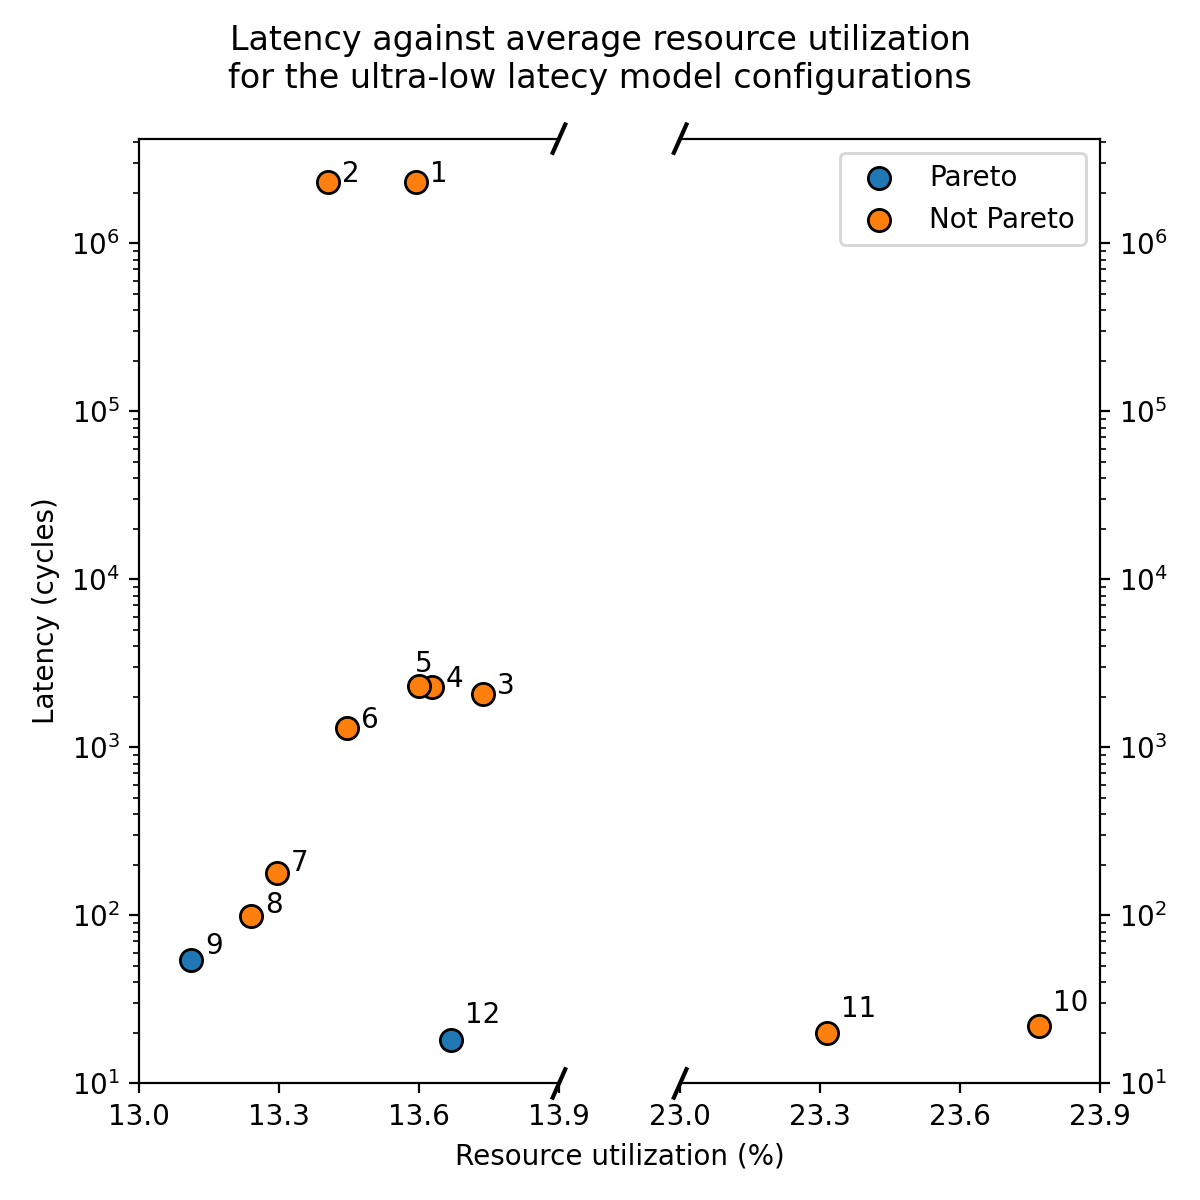
\includegraphics[trim={0cm 0cm 0cm 1.3cm}, clip, width=0.6\textwidth, center]{../logs/hardware_optimizations_pareto.png}
  \caption{Latency plotted against average resource utilization for the ultra-low latency model configurations.}
  \label{fig:hardware-optimizations-pareto}
\end{figure}

\subsection{Verifying Analytical Latency and DSP Models}

The latency estimation formulated in the previous chapter is verified given the synthesis results - the final design requires 18 cycles as predicted. This could only be guaranteed under the assumption that every operation can be completely unrolled and pipelined and all arrays are fully partitioned, which depending on the design might require more resources than there are available. Thanks to the optimizations and simplifications used for the model, this assumption was correct, with the most demanded resource (DSPs) at around a third of its limit.

\begin{equation} \label{eq:dsp-model-new}
  \text{\# of DSPs} = L + C_{\text{linear}} \cdot (21d + 8d^2) + C_{\text{tensor}} \cdot 2 \cdot L^2 \cdot H \approx \mathcal{O}(d^2 + L^2 \cdot H)
\end{equation}

The situation gets more complicated for the DSP model. After a careful analysis of the required hardware footprint of each component of the final design, it turns out that both the linear layer and the tensor product depend on more variables than just their input and output sizes, effectively making the included "constants" vary between instances. It is likely that there exists no easy-to-understand expression, given the complexity of HLS synthesis routing for pipelined designs. In other words, user-independent factors like the order in which HLS processes the design might influence the required hardware resources, including DSPs. However, there is still merit in the proposed model when it comes to its overall computational complexity, as shown in equation \ref{eq:dsp-model-new}. While this does not provide a clear upper boundary for deciding whether a configuration exceeds the available DSP slices, it highlights the quadratic relationship with the latent dimension \(d\), number of input jets \(L\), as well as a linear dependency on the number of self-attention heads \(H\).

\subsection{Accuracy-Focused Model}
The process of creating a hardware model for the accuracy-focused architecture started similarly to previous model. After implementing the necessary layers and changing the design configuration, C simulation reported 


\indo{Talk about grid search for accuracy-focused model as a quick and easy hyperparameter search, that was done mainly to look for simpler designs given very long synthesis, not hardcore tuning accuracy}
\indo{Give estimate of how long is the synthesis and why this is a problem}
\indo{|}
\indo{|}

\begin{figure}[hpt!]
  \centering
  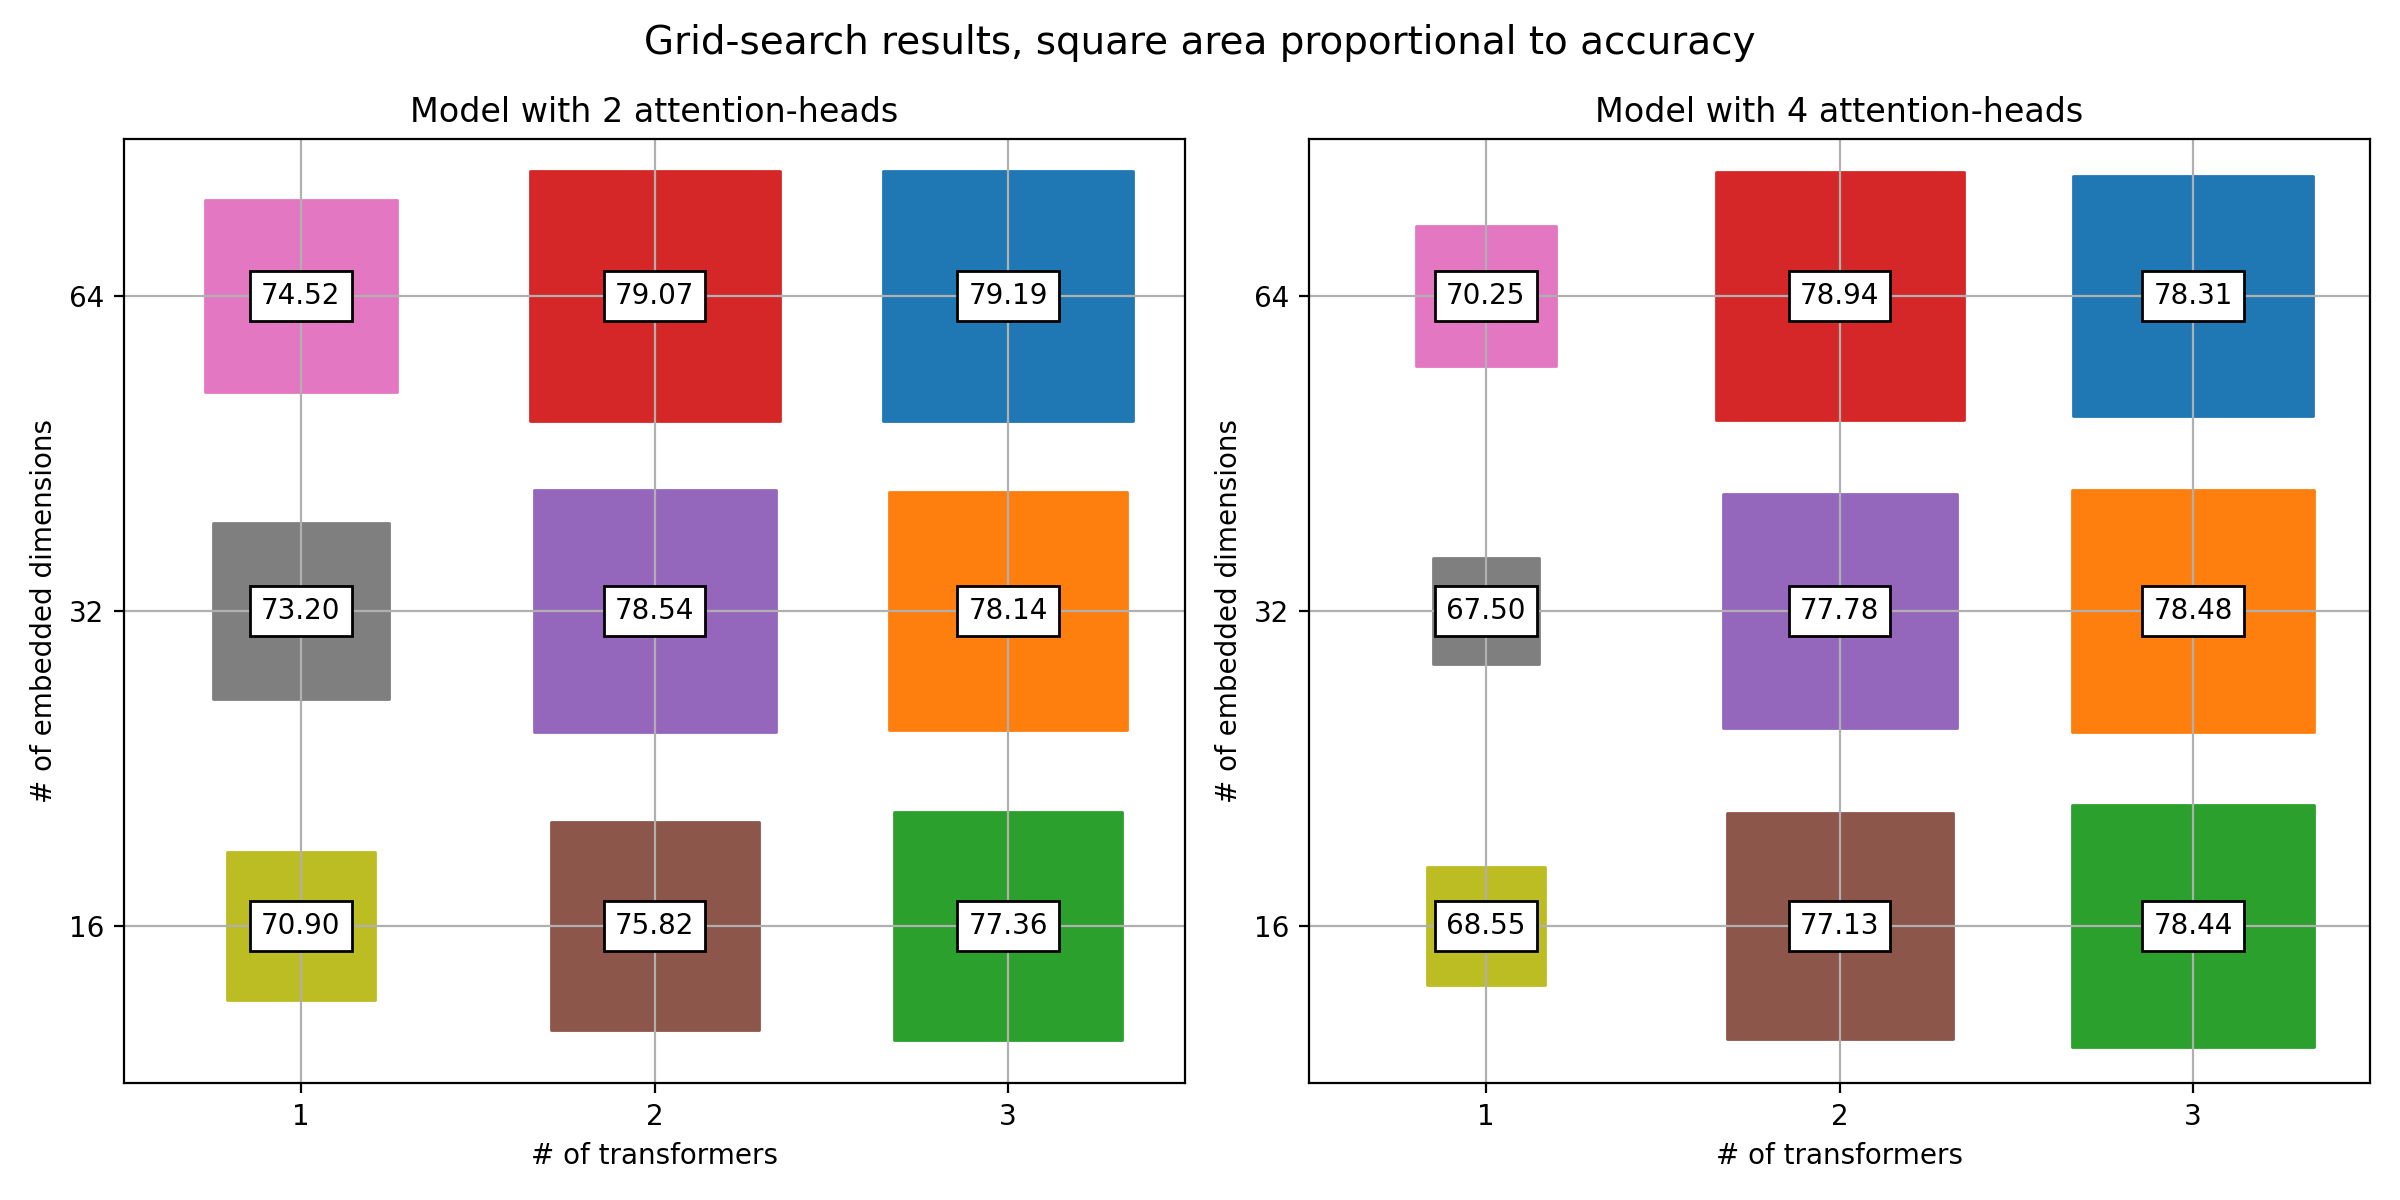
\includegraphics[trim={0cm 0cm 0cm 1cm}, clip, width=1.0\textwidth, center]{../logs/grid_search.png}
  \caption{Grid-search results - squares area proportional to accuracy.}
  \label{fig:grid-search}
\end{figure}

\indo{include table of timing and hardware resources from the non pipelined model}
\indo{do some interpolation based on dense in non pipelined to the one from pipelined by analysing the parameters from ultra low latency and takign care of using too much resources, hene needing to re-use}


\section{Quantization Results}


\subsection{Quantization-Aware Training}
\indo{Recap how this was done and talk about results}
\indo{Mention float16 doesnt learn anything (acc 20\%) as its range is too small, and we cannot consider normalizing inputs as its real time system}
\indo{Mention problems with fixed-point 32 and reason about both int and frac range being important, give examples at which point which one causes issues (likely input -> int range, after normalization -> frac range)}
\indo{Mention brevitas only gets 34\% accuracy and why this is the case and how it could be solved}
\indo{|}
\indo{|}
\indo{|}

\begin{figure}[hpt!]
  \centering
  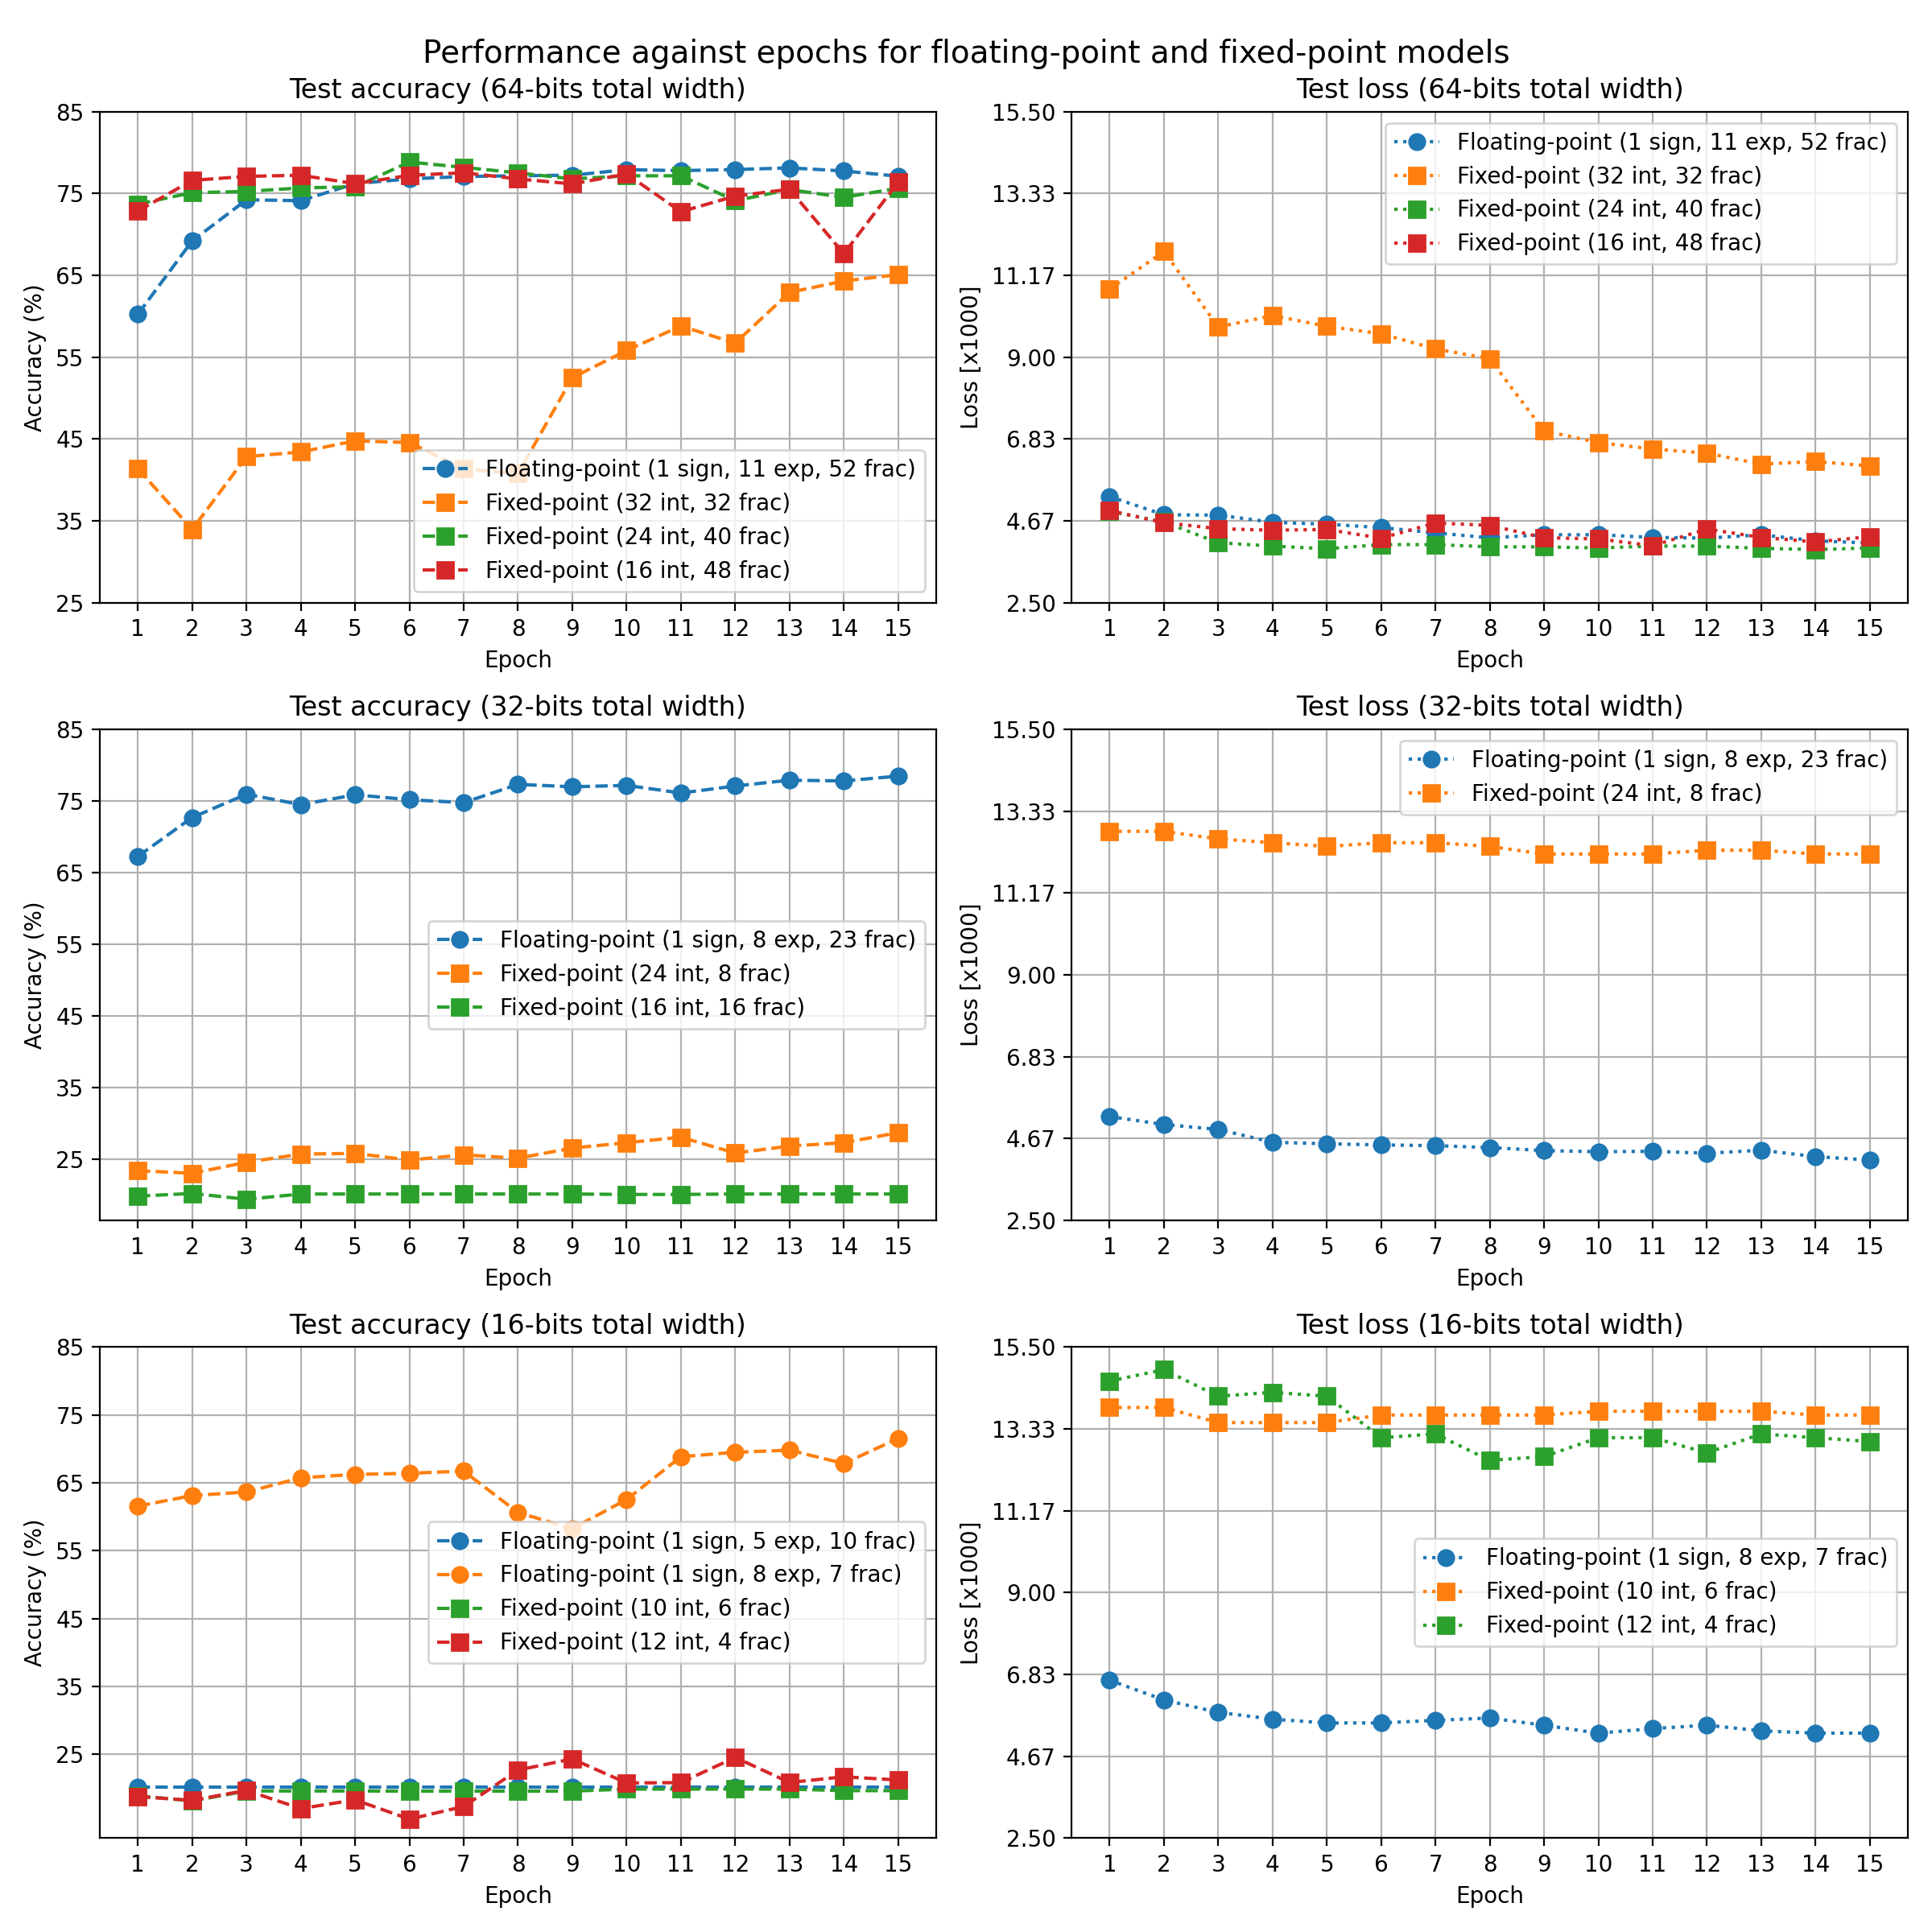
\includegraphics[trim={0cm 0cm 0cm 1.2cm}, clip, width=1.0\textwidth, center]{../logs/training_accuracy.png}
  \caption{Performance against epochs for floating-point and fixed-point models.}
  \label{fig:pre-training}
\end{figure}


\subsection{Post-Training Quantization}\label{eval:post-training-quantization}
\indo{State that the results are very promising (64\% bits reduction), how this should influence synthesis}
\indo{prove correlation with how different on average is the next bit width compared to previous vs default (34 bits etc)}
\indo{say how we dont do synthesis due to time limitations, and its mostly no problem as the widhts are linear with hardware resources aside from the situations in which a dsp can be avoided (34 vs 35 bits etc)}
\indo{Maybe talk about how correlation was verified}
\indo{starting with integer or fractional in the search didnt seem to matter in the limited tests}
\indo{Discuss the used parameters (ratio of positive and negative tolerance etc.) and how they affect the results}
\indo{compare with performance of the HAQ that Walkie suggested}
\indo{|}

\begin{figure}[hpt!]
  \centering
  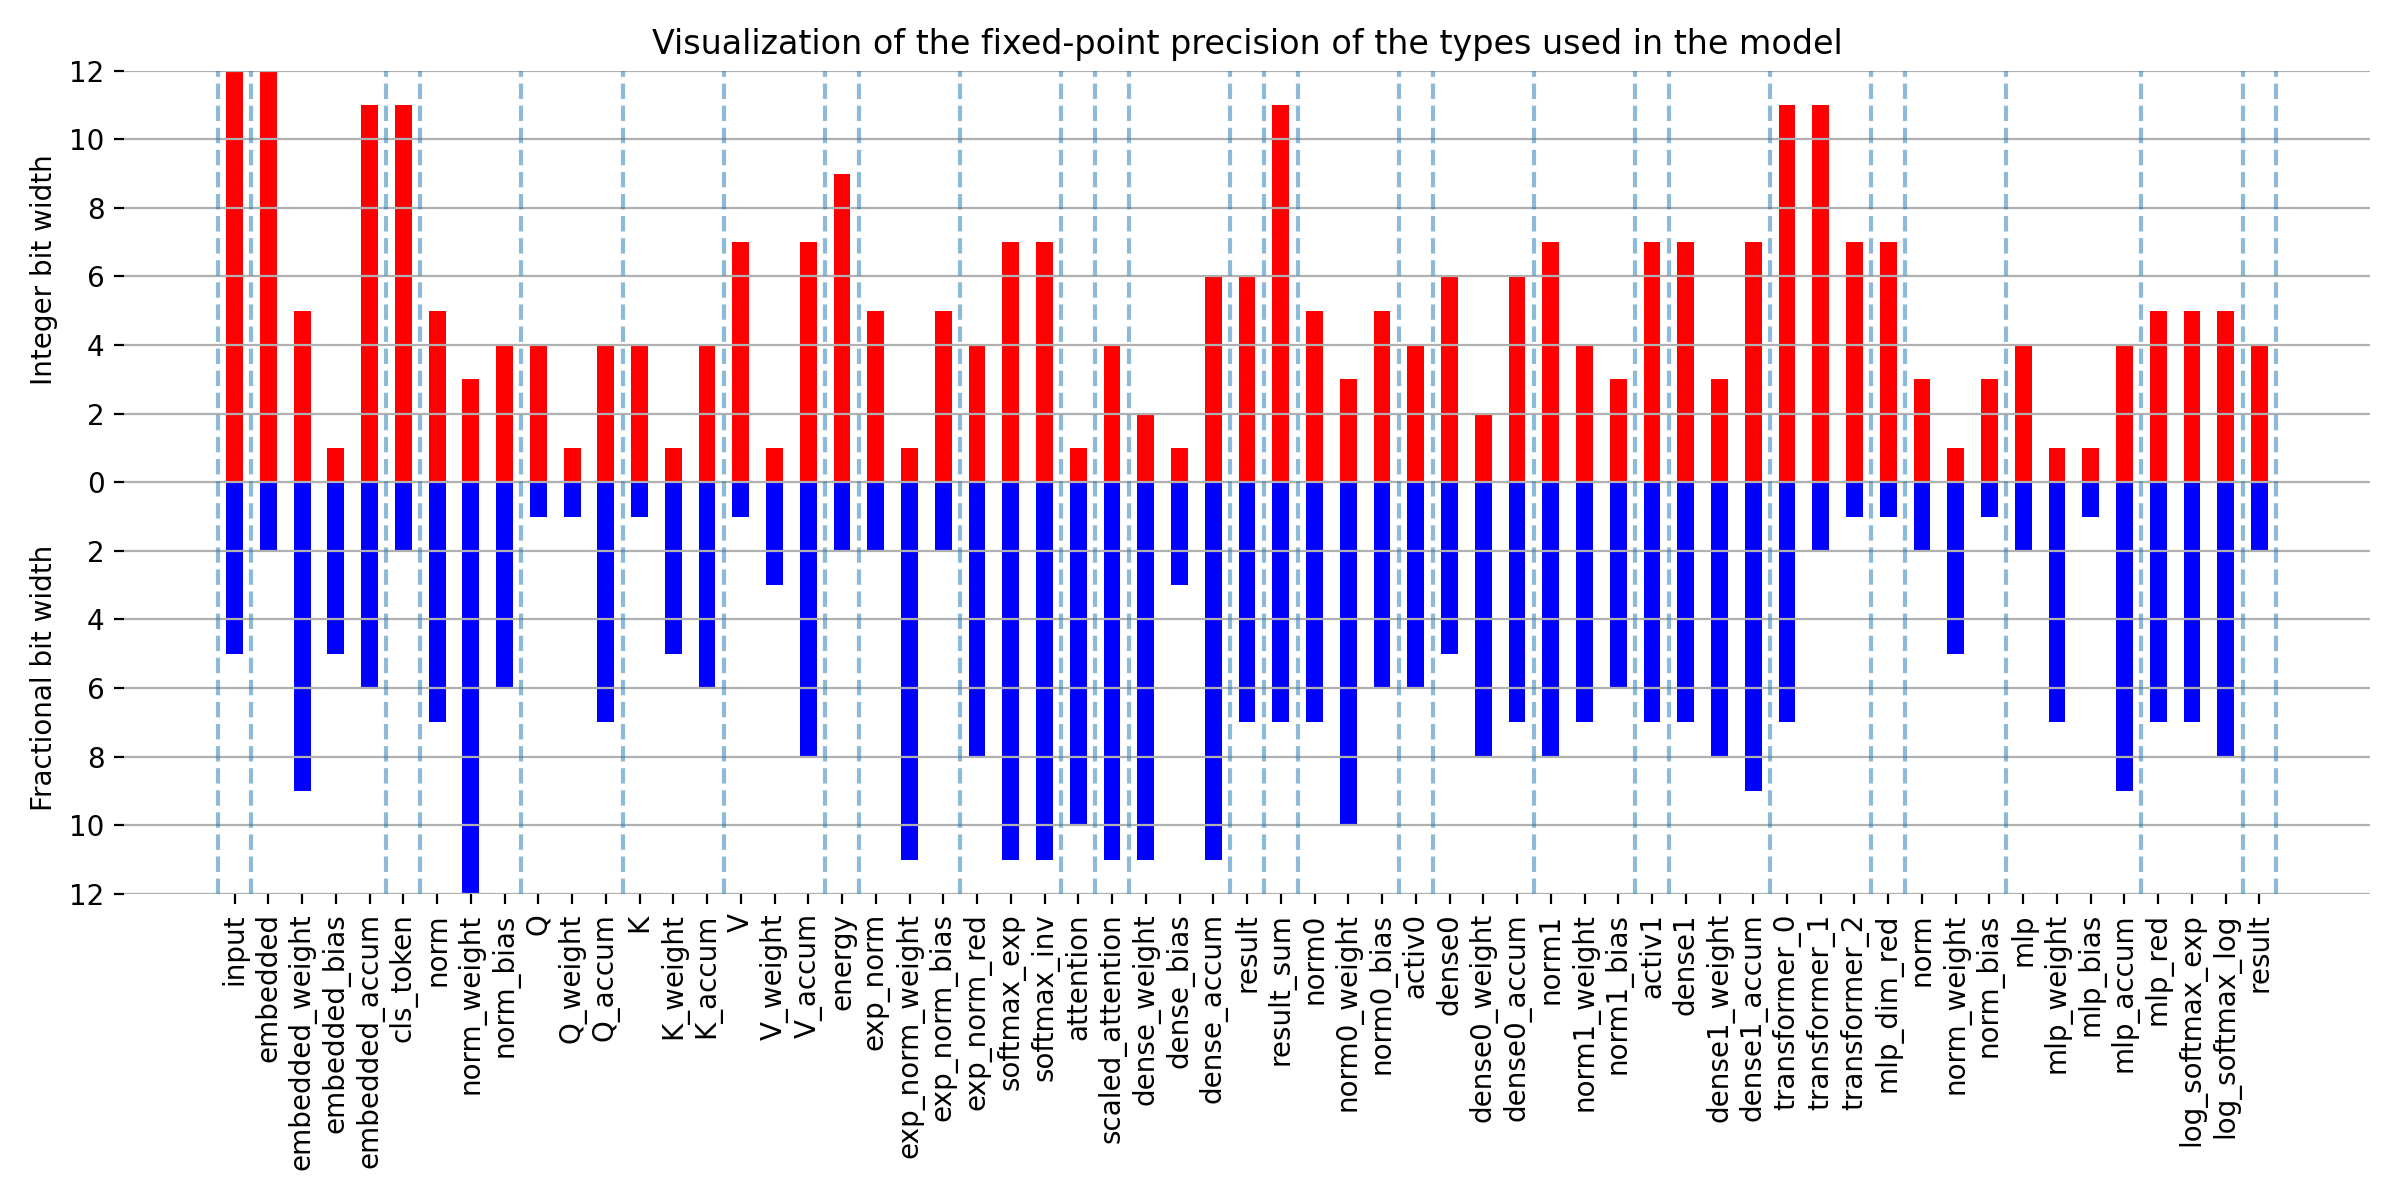
\includegraphics[trim={0cm 0cm 1cm 7.8mm}, clip, width=1.0\textwidth, center]{../logs/bit_width_visualization.png}
  \caption{Visualization of the fixed-point precision of the types used in the accuracy-focused model.}
  \label{fig:post-training-bit-widths}
\end{figure}
